\documentclass{beamer}

\usepackage{xcolor}
\usepackage{graphicx}
\usepackage{booktabs}
\usepackage{array}
\usepackage{amsmath}
\usepackage{tikz}
\usetikzlibrary{arrows.meta,positioning}

\usetheme{Madrid}

\definecolor{mainblue}{RGB}{36,82,140}
\definecolor{accent}{RGB}{0,128,128}
\definecolor{softgray}{RGB}{245,247,250}

\title[BO for EEG Parameter Selection]
{Bayesian Optimisation for Automated Parameter \\ Selection in EEG Feature Extraction}

\author{Fenglin Wang}
\institute[XMUM]{Department of Mathematics\\Xiamen University Malaysia\\[0.12cm]
\small Supervisor: Dr Goh Chien Yong}
\date{June 2026}

\begin{document}
\mode<presentation>

% Main slide 1
\begin{frame}
  \titlepage
\end{frame}


\begin{frame}{Presentation Outline}
  \begin{enumerate}
    \item Background and research problem
    \item Bonn EEG dataset
    \item Proposed methodology
    \item Work completed
    \item Preliminary results
    \item Current findings and next steps
  \end{enumerate}
\end{frame}

\section{Background and Problem}

\begin{frame}{Background and Research Problem}
  \begin{itemize}
    \item EEG classification performance depends strongly on preprocessing
          and feature-extraction parameters.
    \item These parameters are often selected manually through trial and error.
    \item Manual selection may be inefficient and may miss better parameter
          combinations.
    \item The complete five-class Bonn task is challenging, especially for
          the similar interictal classes N and F.
  \end{itemize}

  \begin{block}{Research Problem}
    How can Bayesian Optimisation automate EEG parameter selection and
    improve five-class classification performance?
  \end{block}
\end{frame}


\section{Dataset}

% Main slide 4
\begin{frame}{Bonn EEG Dataset}
  \begin{itemize}
    \item Five classes with 100 EEG segments per class.
    \item Sampling frequency: 173.61 Hz; 4097 samples per segment.
  \end{itemize}

  \begin{table}
    \centering
    \small
    \begin{tabular}{clp{7.2cm}}
      \toprule
      Label & Original set & Recording condition \\
      \midrule
      Z & A & Healthy subjects, eyes open \\
      O & B & Healthy subjects, eyes closed \\
      N & C & Interictal EEG, outside the epileptogenic zone \\
      F & D & Interictal EEG, within the epileptogenic zone \\
      S & E & Ictal EEG during seizure activity \\
      \bottomrule
    \end{tabular}
  \end{table}

\end{frame}

% Main slide 5
\begin{frame}{Project Objectives}
  \begin{enumerate}
    \item Develop an EEG feature-extraction and RBF-SVM classification pipeline.
    \item Apply Bayesian Optimisation to preprocessing and SVM parameters.
    \item Compare BO-SVM with a manually configured SVM and Random Search.
    \item Analyze preliminary five-class errors, especially confusion between N and F.
  \end{enumerate}

  \begin{block}{Role of Five-Class Classification}
    The Z/O/N/F/S task is used as an experimental platform for evaluating parameter-selection methods.
  \end{block}
\end{frame}

\section{Proposed Methodology}


\begin{frame}{Proposed BO-SVM Pipeline}
  \centering
  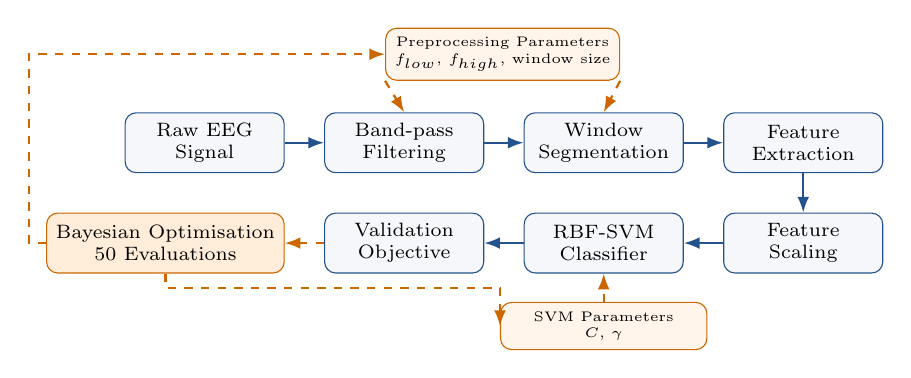
\begin{tikzpicture}[
    node distance=0.50cm,
    box/.style={draw=mainblue, rounded corners, align=center,
      minimum width=2.02cm, minimum height=0.76cm,
      fill=softgray, font=\scriptsize},
    bo/.style={draw=orange!80!black, rounded corners, align=center,
      minimum width=2.05cm, minimum height=0.76cm,
      fill=orange!15, font=\scriptsize},
    param/.style={draw=orange!80!black, rounded corners, align=center,
      minimum width=2.62cm, minimum height=0.56cm,
      fill=orange!8, font=\tiny},
    flow/.style={-{Latex[length=2mm]}, thick, mainblue},
    control/.style={-{Latex[length=2mm]}, thick, dashed, orange!80!black}
  ]
    \node[box] (raw) {Raw EEG\\Signal};
    \node[box, right=of raw] (filter) {Band-pass\\Filtering};
    \node[box, right=of filter] (window) {Window\\Segmentation};
    \node[box, right=of window] (feature) {Feature\\Extraction};
    \node[box, below=of feature] (scaling) {Feature\\Scaling};
    \node[box, left=of scaling] (svm) {RBF-SVM\\Classifier};
    \node[box, left=of svm] (objective) {Validation\\Objective};
    \node[bo, left=of objective] (bo) {Bayesian Optimisation\\50 Evaluations};

    \node[param, above=0.40cm of filter, xshift=1.25cm]
      (preparam) {Preprocessing Parameters\\
      $f_{low}$, $f_{high}$, window size};
    \node[param, below=0.36cm of svm]
      (svmparam) {SVM Parameters\\$C$, $\gamma$};

    \draw[flow] (raw) -- (filter);
    \draw[flow] (filter) -- (window);
    \draw[flow] (window) -- (feature);
    \draw[flow] (feature) -- (scaling);
    \draw[flow] (scaling) -- (svm);
    \draw[flow] (svm) -- (objective);
    \draw[control] (objective) -- (bo);
    \draw[control] (bo.west) -- ++(-0.22,0) |- (preparam.west);
    \draw[control] (bo.south) -- ++(0,-0.18) -| (svmparam.west);
    \draw[control] (preparam.south west) -- (filter.north);
    \draw[control] (preparam.south east) -- (window.north);
    \draw[control] (svmparam.north) -- (svm.south);
  \end{tikzpicture}

  \vspace{0.16cm}
  \begin{block}{Optimisation Loop}
    BO proposes a parameter combination, the EEG-SVM pipeline returns a validation score, and that score guides the next evaluation.
  \end{block}
\end{frame}

\begin{frame}{PSD Feature Configuration}

  \begin{columns}[T,onlytextwidth]

    \begin{column}{0.48\textwidth}
      \begin{block}{Welch PSD Estimation}
        \footnotesize
        \begin{itemize}
          \setlength{\itemsep}{0.25em}
          \setlength{\parskip}{0pt}
          \item Hann window
          \item $n_{\mathrm{perseg}}=\min(256,N_w)$
          \item 50\% internal Welch overlap
          \item Constant detrending
          \item Density scaling
        \end{itemize}
      \end{block}
    \end{column}

    \begin{column}{0.48\textwidth}
      \begin{block}{EEG Frequency Bands}
        \centering
        \footnotesize
        \begin{tabular}{lc}
          \toprule
          Band & Frequency range \\
          \midrule
          Delta & 0.5--4 Hz \\
          Theta & 4--8 Hz \\
          Alpha & 8--13 Hz \\
          Beta  & 13--30 Hz \\
          Gamma & 30--40 Hz \\
          \bottomrule
        \end{tabular}
      \end{block}
    \end{column}

  \end{columns}

  \vspace{0.1cm}

  \begin{block}{Extracted PSD Features}
    \footnotesize
    \begin{columns}[T,onlytextwidth]
      \begin{column}{0.32\textwidth}
        \centering
        Absolute band power
      \end{column}

      \begin{column}{0.32\textwidth}
        \centering
        Relative band power
      \end{column}

      \begin{column}{0.32\textwidth}
        \centering
        Selected band-power ratios
      \end{column}
    \end{columns}
  \end{block}

  \vspace{0.05cm}

  {\scriptsize
  For window length $T$,
  $N_w=\operatorname{round}(173.61T)$.
  Incomplete trailing samples are discarded.
  Relative power emphasizes spectral distribution and reduces the
  influence of overall signal amplitude.
  }

\end{frame}




\begin{frame}{Feature Extraction: 55 Features per Window}
  \scriptsize
  \begin{columns}[T]
    \begin{column}{0.48\textwidth}
      \begin{block}{Feature Composition}
        \begin{table}
          \centering
          \scriptsize
          \begin{tabular}{lc}
            \toprule
            Feature group & Dimension \\
            \midrule
            Absolute band power & 5 \\
            Relative band power & 5 \\
            Band-power ratios & 6 \\
            Statistical features & 13 \\
            Entropy features & 3 \\
            Hjorth parameters & 3 \\
            DWT features & 20 \\
            \midrule
            Total & \textbf{55} \\
            \bottomrule
          \end{tabular}
        \end{table}
      \end{block}
    \end{column}

    \begin{column}{0.48\textwidth}
      \begin{block}{Approximate Entropy}
        \begin{itemize}
          \item Embedding dimension: $m=2$
          \item Tolerance: $r=0.2\sigma$
          \item Maximum input length: 80 points
          \item Longer windows are uniformly downsampled
          \item $\mathrm{ApEn}=\phi(2)-\phi(3)$
        \end{itemize}
      \end{block}

      \begin{block}{Additional Features}
        \begin{itemize}
          \item Entropy: Shannon, spectral and approximate
          \item Hjorth: activity, mobility and complexity
          \item DWT: db4, level 3, four coefficient sets
          \item Five DWT descriptors per coefficient set
        \end{itemize}
      \end{block}
    \end{column}
  \end{columns}
\end{frame}

% Main slide 9
\begin{frame}{Why RBF-SVM and Bayesian Optimisation?}
  \begin{columns}[T]
    \begin{column}{0.48\textwidth}
      \begin{block}{Why RBF-SVM?}
        \begin{itemize}
          \item Suitable for a relatively small dataset
          \item Models nonlinear class boundaries
          \item Works with handcrafted feature vectors
        \end{itemize}
      \end{block}
    \end{column}

    \begin{column}{0.48\textwidth}
      \begin{block}{Why BO?}
        \begin{itemize}
          \item Manual selection may miss useful combinations
          \item Previous evaluations guide the next trial
          \item Suitable for expensive black-box objectives
        \end{itemize}
      \end{block}
    \end{column}
  \end{columns}

  \vspace{0.25cm}
  \centering
  \small BO uses a Gaussian-process surrogate and Expected Improvement.\\
  \scriptsize Based on Snoek et al. (2012).
\end{frame}


\begin{frame}{Current BO Experimental Setup}
  \begin{columns}[T]
    \begin{column}{0.47\textwidth}
      \begin{table}
        \centering
        \scriptsize
        \begin{tabular}{ll}
          \toprule
          Parameter & Current range \\
          \midrule
          $f_{low}$ & 0.5--5.0 Hz \\
          $f_{high}$ & 30--60 Hz \\
          Window size & 1--5 s \\
          $C$ & 0.1--100 \\
          $\gamma$ & $10^{-4}$--1 \\
          \bottomrule
        \end{tabular}
      \end{table}
    \end{column}

    \begin{column}{0.49\textwidth}
      \begin{block}{BO Components}
        \begin{itemize}
          \item GP surrogate: Mat\'ern kernel
          \item Acquisition: Expected Improvement
          \item Class weighting: balanced
          \item BO/Random Search budget: 50 evaluations
        \end{itemize}
      \end{block}
    \end{column}
  \end{columns}

  \[
    \text{Score} =
    0.35\,\text{Accuracy}
    +0.25\,\text{Macro Recall}
    +0.20\,\text{Recall}_{N}
    +0.20\,\text{Recall}_{F}
  \]

  \scriptsize The extra N/F terms reflect the current difficulty observed in the five-class task.
  The 80/20 outer split is performed by original EEG segment; optimisation
  uses five-fold StratifiedGroupKFold and the held-out test set is evaluated once.
\end{frame}

\section{Preliminary Results}


\section{Current Progress}

\begin{frame}{Work Completed }
  \begin{itemize}
    \item Organized and verified the five Bonn EEG subsets.
    \item Developed the filtering, windowing and feature-extraction pipeline.
    \item Implemented PSD, statistical, entropy and Hjorth features.
    \item Established a scaled RBF-SVM baseline.
    \item Implemented Bayesian Optimisation and Random Search.
    \item Completed a grouped five-class comparison using 50 BO and Random Search evaluations.
  \end{itemize}

  \begin{block}{Current Status}
    Manual SVM, Random Search and BO now use the same grouped split,
    feature pipeline, validation folds, scaling and final test procedure.
  \end{block}
\end{frame}

\begin{frame}{Preliminary Five-Class Results}
  \begin{columns}
    \begin{column}{0.43\textwidth}
      \begin{table}
        \centering
        \small
        \begin{tabular}{lc}
          \toprule
          Method & Accuracy \\
          \midrule
          Manual SVM & 76.45\% \\
          Random Search & 81.20\% \\
          BO-SVM & \textbf{84.75\%} \\
          \bottomrule
        \end{tabular}
      \end{table}
    \end{column}

    \begin{column}{0.55\textwidth}
      \centering
      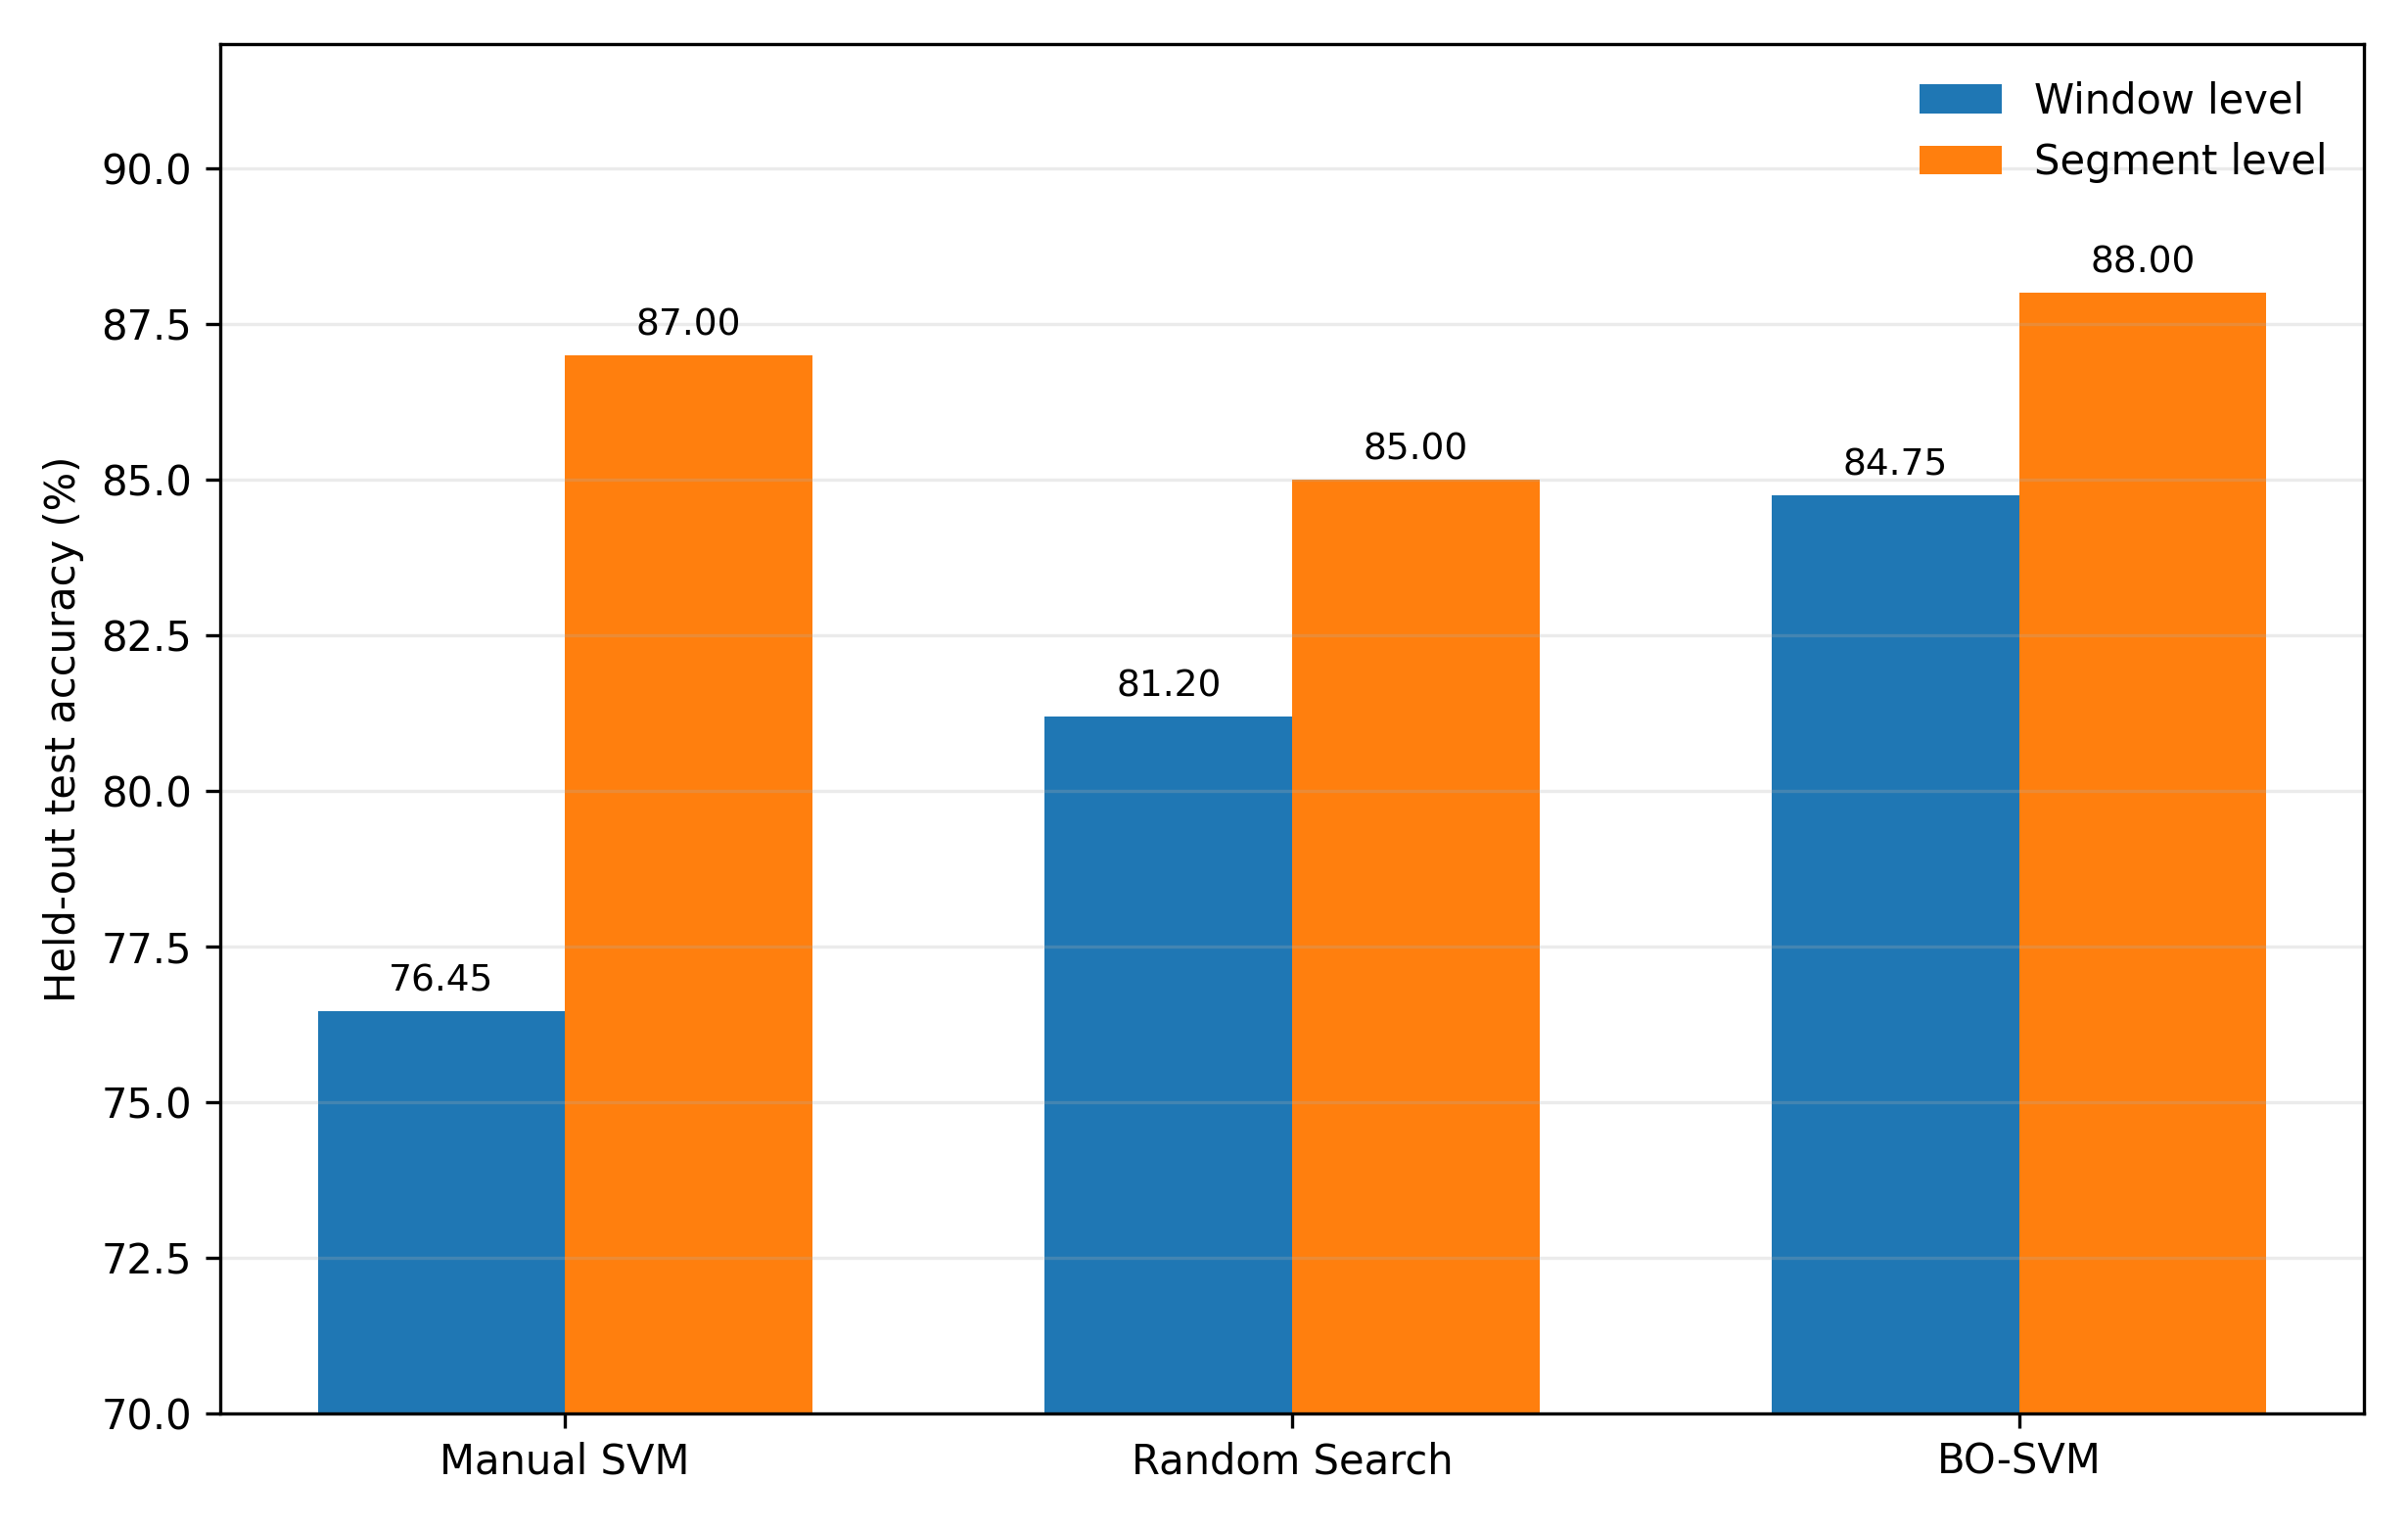
\includegraphics[width=\textwidth]{results/04_grouped_bo_svm/grouped_method_accuracy_comparison.png}
    \end{column}
  \end{columns}

  \begin{block}{Preliminary Interpretation}
    BO-SVM achieved the highest accuracy in this single grouped run.
    Its 3.55 percentage-point advantage over Random Search requires
    confirmation using repeated grouped evaluations.
  \end{block}

  \scriptsize Window-level held-out test accuracy; each method accessed the test set once.
\end{frame}


\begin{frame}{Current Best BO-SVM Configuration and Performance}

  \begin{table}
    \centering
    \scriptsize
    \begin{tabular}{lc@{\hspace{1.2cm}}lc}
  \toprule
  BO parameter & Selected value & Other information & Value \\
  \midrule
  $f_{low}$   & 0.5 Hz & Class weight & balanced \\
  $f_{high}$  & 60.0 Hz  & Input features per window & 55 \\
  Window size & 5.0 s    & Best evaluation & 20/50 \\
  $C$         & 7.6716   & Grouped CV folds & 5 \\
  $\gamma$    & 0.023208 & Test evaluations & 1 \\
  \bottomrule
\end{tabular}
  \end{table}

  \vspace{-0.1cm}
  \centering
  
  \vspace{0.15cm}

  \begin{columns}[t]
    \begin{column}{0.43\textwidth}
      \centering
      {\small\textbf{Overall and Class-Wise Performance}}
      \begin{table}
        \scriptsize
        \begin{tabular}{lc}
          \toprule
          Metric & Value \\
          \midrule
          Accuracy & 84.75\% \\
          Macro recall & 84.75\% \\
          Recall Z & 92.50\% \\
          Recall O & 88.75\% \\
          Recall N & 83.75\% \\
          Recall F & \textbf{63.75\%} \\
          Seizure sensitivity & \textbf{95.00\%} \\
          \bottomrule
        \end{tabular}
      \end{table}
    \end{column}

    \begin{column}{0.53\textwidth}
      \centering
      {\small\textbf{Confusion Matrix}}
      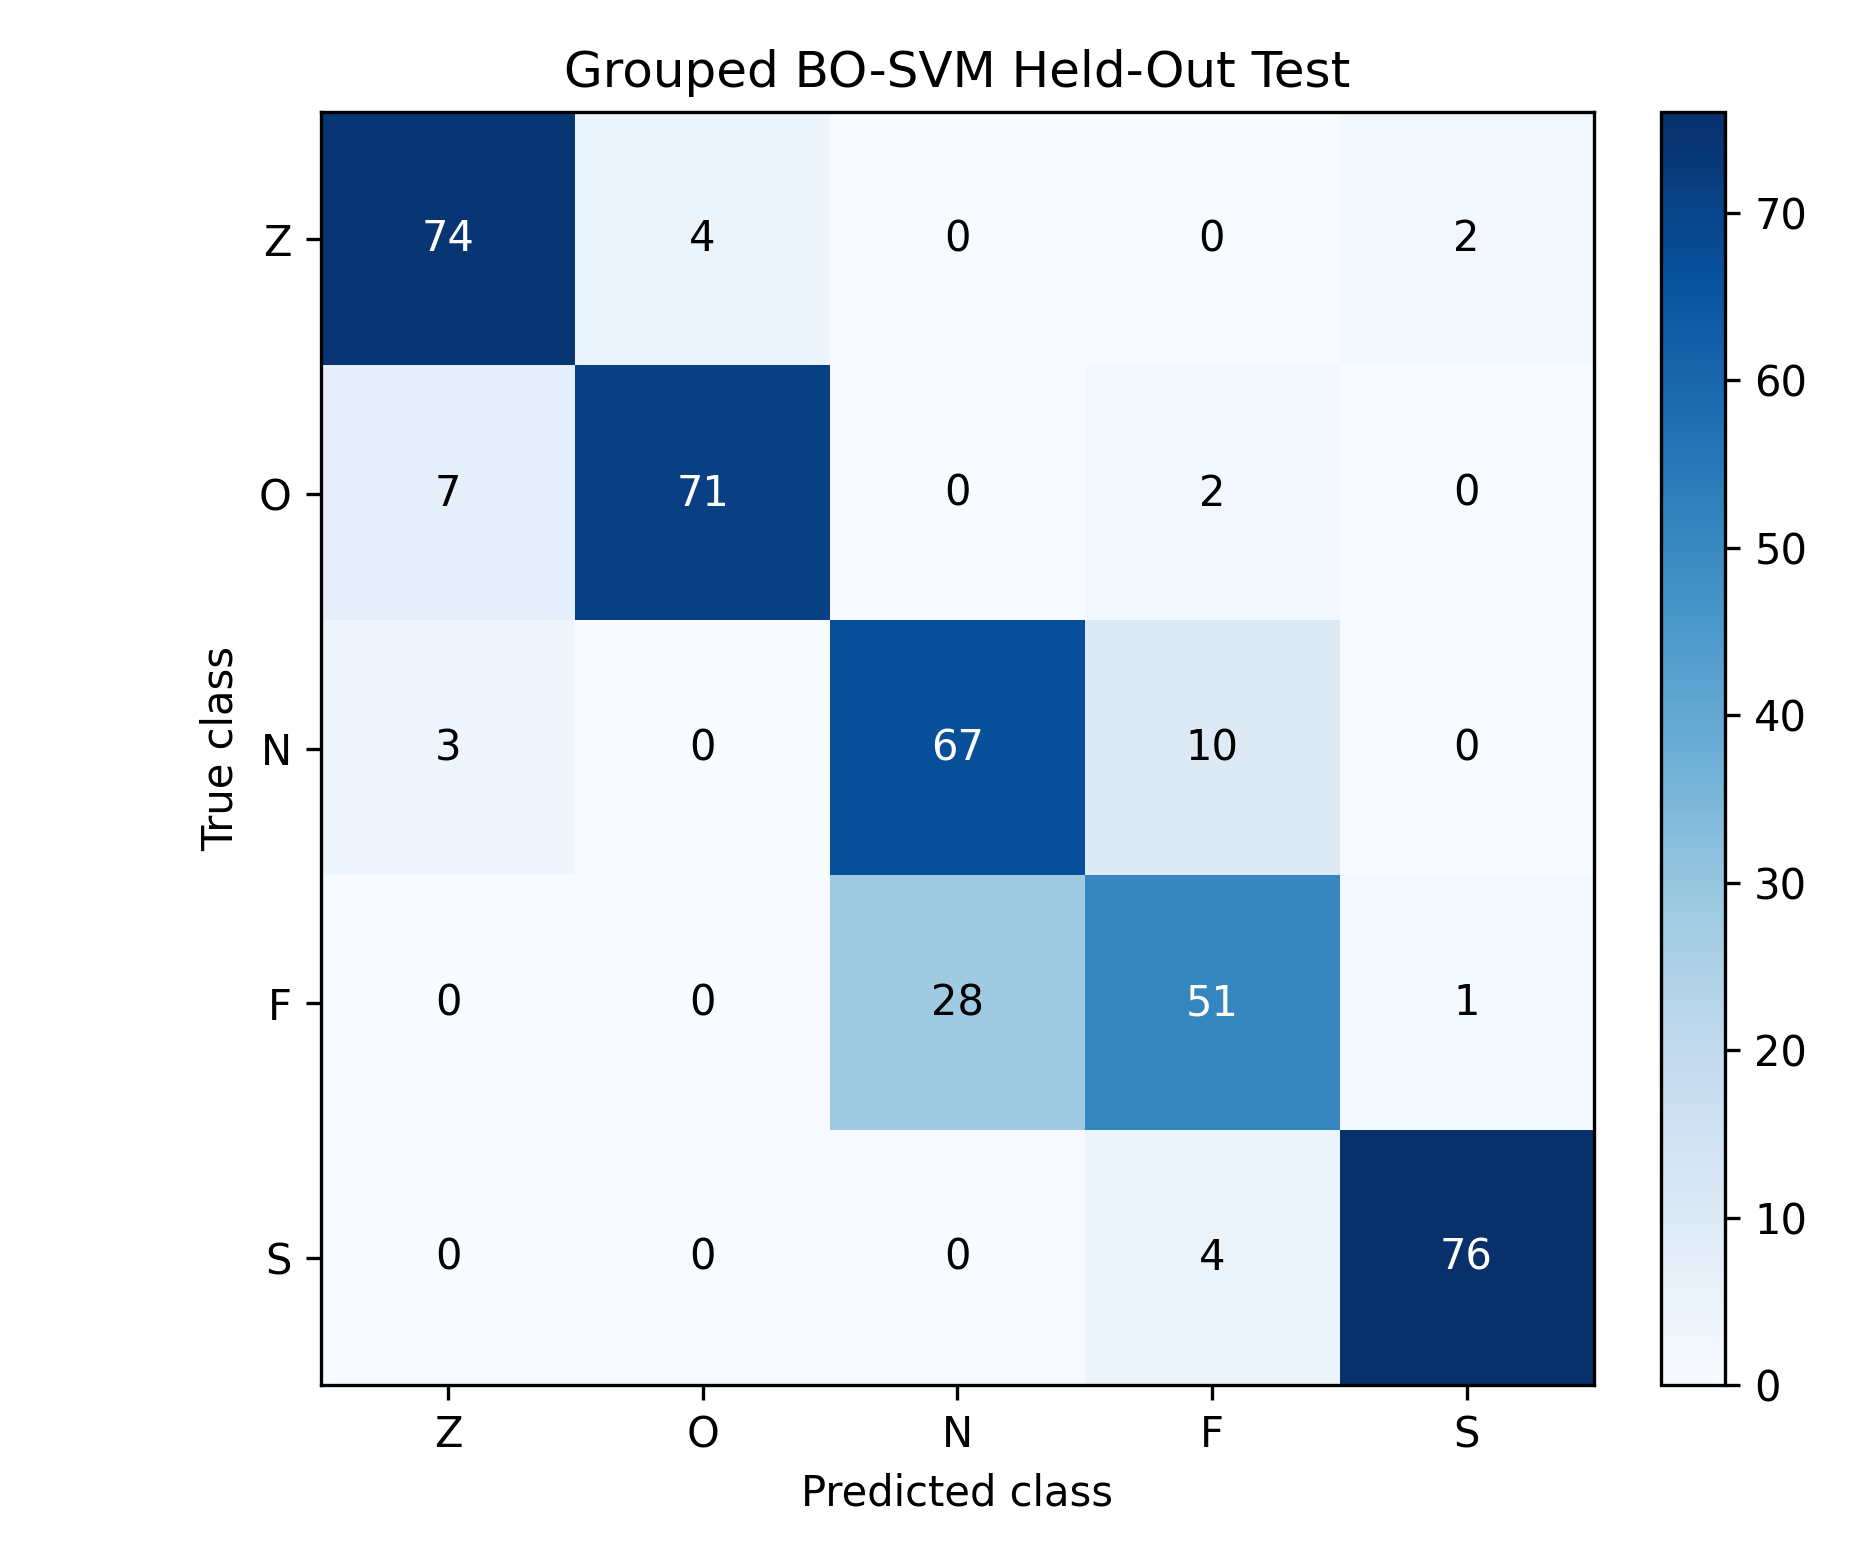
\includegraphics[width=0.86\textwidth]
      {results/04_grouped_bo_svm/grouped_bo_test_confusion_matrix.png}

      \scriptsize Grouped BO-SVM held-out test confusion matrix
    \end{column}
  \end{columns}

\end{frame}





\begin{frame}{BO and Random Search Progress}
  \begin{columns}
    \begin{column}{0.58\textwidth}
      \centering
      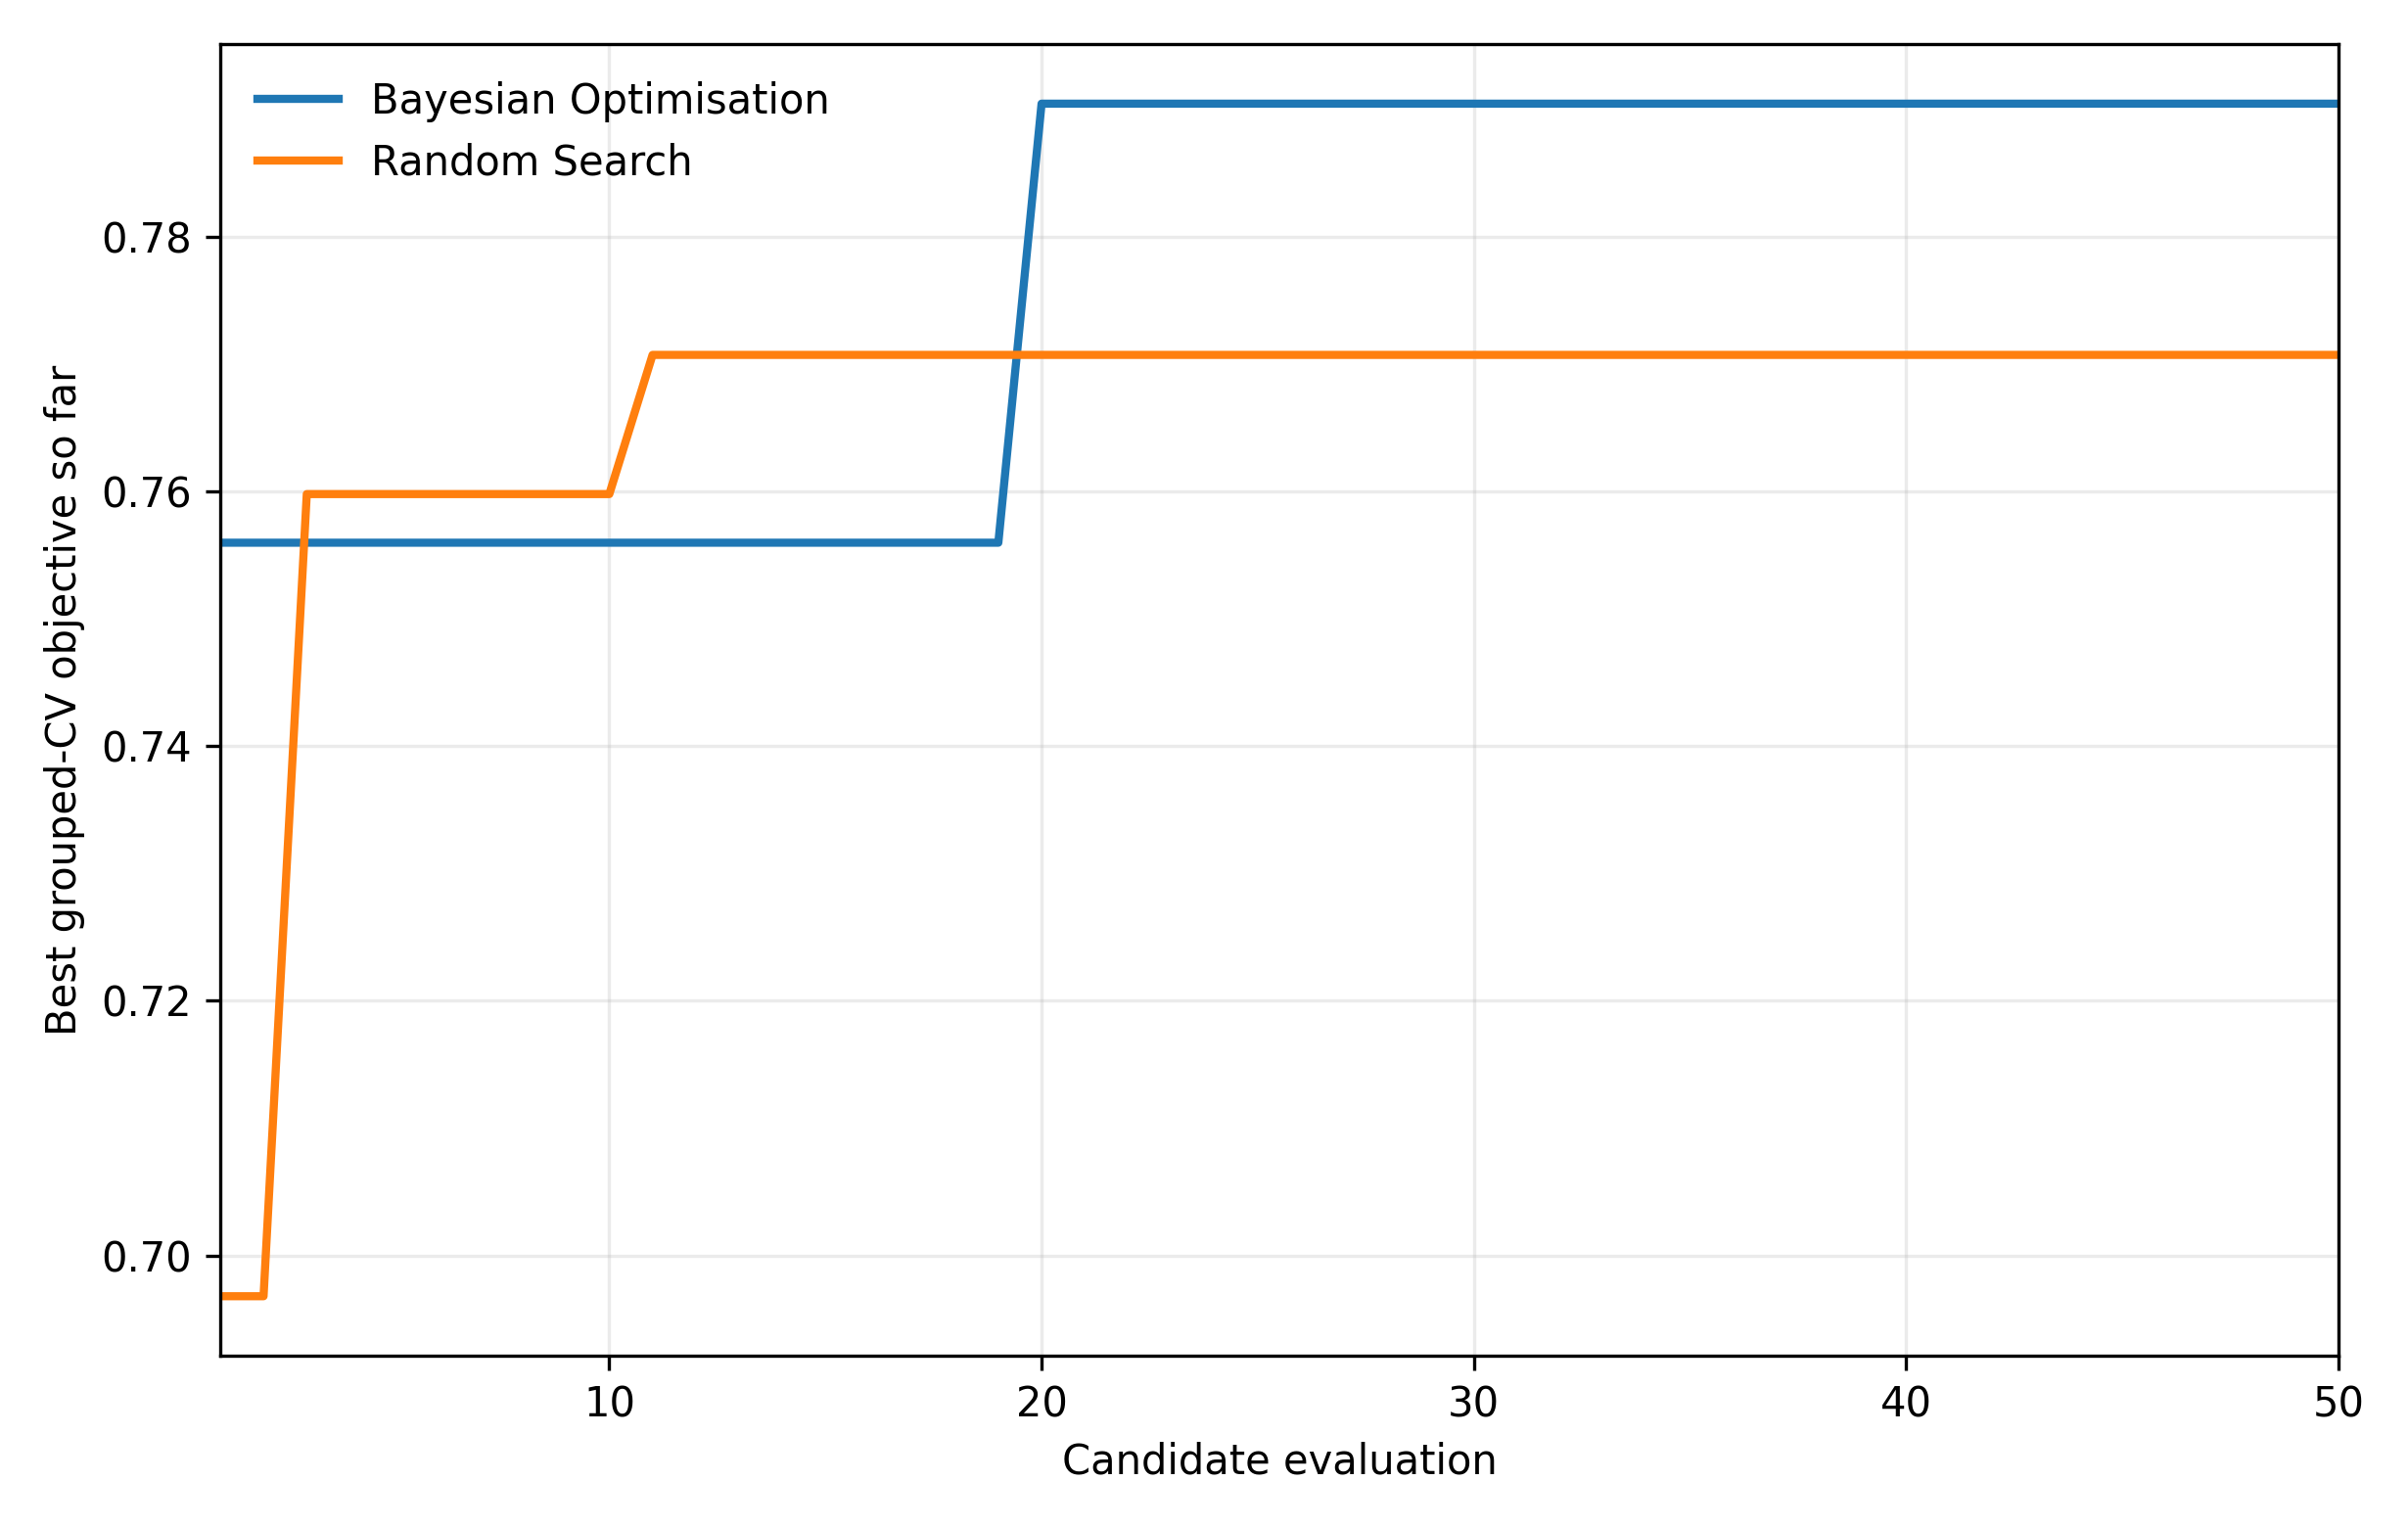
\includegraphics[width=\textwidth]{results/04_grouped_bo_svm/grouped_bo_vs_random_convergence.png}
      \scriptsize Best grouped-CV objective observed so far
    \end{column}

    \begin{column}{0.39\textwidth}
      \begin{itemize}
      \item Each curve uses the same search space and 50-evaluation budget.
      \item BO uses a GP surrogate and Expected Improvement.
      \item The held-out test set is not used by either curve.
    \end{itemize}
    \end{column}
  \end{columns}

  \begin{block}{Preliminary Observation}
    BO found the highest grouped-CV objective at evaluation 20, while
    Random Search found its best candidate at evaluation 11.
  \end{block}
\end{frame}


\begin{frame}{Evaluation Criteria for Supplementary Subset Tasks}

  \begin{block}{BO Selection Criterion}
    \scriptsize
    For the supplementary subset tasks, BO selected the best parameter
    setting mainly using validation accuracy.
  \end{block}

  \begin{block}{Reported Metrics}
    \scriptsize
    After the best setting was selected, the held-out test results were
    reported using:
    \begin{itemize}
      \item Accuracy and macro recall
      \item Seizure recall, treating class S as the positive class
      \item Seizure specificity, treating all non-S classes as negative
    \end{itemize}
  \end{block}

  \begin{block}{Reason for This Setting}
    \scriptsize
    These tasks were simpler binary or three-class subset problems,
    including Z vs S, F vs S, and Z vs F vs S. The aim was to check whether
    the same BO-SVM pipeline could separate seizure-related patterns under
    reduced class structures, rather than to optimise the difficult N/F
    confusion in the full five-class task.
  \end{block}

\end{frame}


\begin{frame}{Supplementary Binary and Three-Class Results}
  \begin{table}
    \centering
     \small
    \begin{tabular}{lcc}
      \toprule
      Task & Accuracy & Seizure recall (class S)  \\
      \midrule
      Z vs S (A--E) & 99.00\% & 98.00\% \\
      F vs S (D--E) & 99.72\% & 99.44\% \\
      Z vs F vs S (A--D--E) & 97.08\% & 99.38\% \\
      \bottomrule
    \end{tabular}
  \end{table}

 \begin{block}{Key Observation}
  The reduced-class tasks achieve high seizure recall, while the complete
  five-class task remains more challenging.
\end{block}

\scriptsize
Class S is treated as the positive class. BO setting: 20 evaluations with
16 initial points for each supplementary task. These earlier subset results
use a window-level split and are not directly comparable with the grouped
five-class experiment.
\end{frame}

\begin{frame}{Preliminary Literature Comparison}
  \begin{table}
    \centering
    \scriptsize
    \resizebox{\textwidth}{!}{%
    \begin{tabular}{p{2.5cm}p{3.5cm}p{3.5cm}p{4.5cm}}
      \toprule
      Study & Bonn task & Method & Reported result \\
      \midrule

      Gupta et al. (2021)
      & Five-class; binary $(Z+O)$ vs $S$
      & One-dimensional neural network with skip connections
      & Five-class: 81.0\% average sensitivity and 81.4\%
        average precision; binary: 99.5\% sensitivity and
        99.9\% precision\\

      Guharoy et al. (2024)
      & Six binary pairs: A--C, A--D, A--E, B--C, B--D and B--E
      & DWT + ICA + SVM
      & 90.42\% mean accuracy using 10-fold cross-validation \\

      \bottomrule
    \end{tabular}%
    }
  \end{table}

  \begin{block}{Interpretation Boundary}
    These results provide contextual references rather than a direct
    leaderboard because the class combinations, metrics and evaluation
    protocols differ.
  \end{block}
 \end{frame}

\section{Conclusion}
\begin{frame}{Current Limitations}
  \begin{itemize}
    \item The current grouped comparison uses one outer split and one random seed.
    \item Segment-level predictions use majority voting across windows.
    \item The evaluation is segment-independent, but not subject-independent.
    \item Class F recall remains lower than the other classes.
  \end{itemize}

  \begin{block}{Interpretation Boundary}
    Grouped splitting prevents windows from the same EEG segment crossing
    data partitions, but it does not establish subject-independent or clinical generalisation.
  \end{block}
\end{frame}

\begin{frame}{Summary and Next Steps}
  \begin{block}{Current Progress}
    \begin{itemize}
      \item A grouped EEG feature-extraction and RBF-SVM pipeline has been implemented.
      \item Manual SVM, Random Search and BO now use the same evaluation protocol.
      \item BO achieved 84.75\% window-level and 88.00\% segment-level accuracy.
      \item N/F separation remains the main classification challenge.
    \end{itemize}
  \end{block}

  \begin{block}{Next Steps}
    \begin{itemize}
      \item Repeat the full grouped comparison using multiple random seeds.
      \item Report mean $\pm$ standard deviation or confidence intervals.
      \item Further investigate features for improving N/F separation.
    \end{itemize}
  \end{block}
\end{frame}


\begin{frame}{References}
  \scriptsize
  \begin{thebibliography}{9}
    \bibitem{Andrzejak2001}
    R. G. Andrzejak et al. (2001).
    \newblock Indications of nonlinear deterministic and finite-dimensional structures in time series of brain electrical activity.
    \newblock \emph{Physical Review E}, 64(6), 061907.

    \bibitem{Snoek2012}
    J. Snoek, H. Larochelle, and R. P. Adams (2012).
    \newblock Practical Bayesian Optimization of Machine Learning Algorithms.
    \newblock \emph{Advances in Neural Information Processing Systems}, 25.

    \bibitem{Gupta2021}
    S. Gupta, J. Meena, and O. P. Gupta (2021).
    \newblock Neural Network Based Epileptic EEG Detection and Classification.
    \newblock arXiv:2111.03268.

    \bibitem{Guharoy2021}
    R. Guharoy, N. D. Jana, and S. Biswas (2021).
    \newblock An Efficient Epileptic Seizure Detection Technique using Discrete Wavelet Transform and Machine Learning Classifiers.
    \newblock arXiv:2109.13811v2.

    \bibitem{Guharoy2024}
    R. Guharoy et al. (2024).
    \newblock Novel Epileptic Seizure Detection Techniques and their Empirical Analysis.
    \newblock arXiv:2302.12012v4.
  \end{thebibliography}
\end{frame}

\end{document}
